\documentclass[9pt,conference]{IEEEtran}
\usepackage{cite}
\usepackage{amsmath,amssymb,amsfonts}
\usepackage{multirow}
\usepackage{array}
\usepackage{graphicx}
\usepackage{textcomp}
\usepackage{xcolor}
\usepackage{algorithm}
\usepackage[noend]{algpseudocode}
\usepackage{hhline}
\usepackage{mathrsfs}
\usepackage{float}
\graphicspath{{Figures/}}

\begin{document}

\title{Experiment: 1\\Study of voltage multiplier using
clamper and peak detector circuit}

\author{
    \IEEEauthorblockA{Siddhant Shah (B23334) *, Akash Goel(B23032) †, 
                      Om Maheshwari (B23089) ‡, and Somya Bhadada (B23052) §}
* b23334@students.iitmandi.ac.in \\
† b23032@students.iitmandi.ac.in \\
‡ b23089@students.iitmandi.ac.in \\
§ b23052@students.iitmandi.ac.in}
\date{}

\maketitle


\begin{abstract}
\noindent{This report presents the study and implementation of voltage multipliers using clamper and peak detector circuits.Also, First we implement the clamper and peak detector circuits alone then we approach towards the implementation of voltage doubler \& quadruple. The results obtained in the form of CSV file are then plotted using MATLAB. The results obtained from practical implementation are compared with theoretical expectations.}
\end{abstract}

\section{Components Required}
\begin{itemize}
    \item Diode – IN4007
    \item Signal generator
    \item Capacitor 10uF
    \item Breadboard, wires, CRO, and multimeter for testing
\end{itemize}

\section{Theory}
\subsection{Clamper Theory}
\noindent{A clamper is a circuit that "clamps" a signal to a different DC level without changing the appearance of the applied signal. The different types of clampers are positive, negative, and biased clampers. A clamping network must have at least a capacitor and a diode.}

\subsection{Peak Detector}
\noindent{Peak detector circuits determine the peak (maximum) value of an input signal. It stores the peak value of input voltages for an infinite duration until reset. The peak detector circuit follows the highest value of an input signal and stores it.}

\subsection{Voltage Multiplier}
\noindent{Voltage multiplier circuits are used to generate a higher DC voltage from an AC input without a transformer. They achieve this by using a network of diodes and capacitors to rectify and store charge, progressively increasing the output voltage in stages.}

\section{Results}
\subsection{Clamper Circuit}
\begin{itemize}
    \item Implemented clamper circuit for an input voltage of 5Vpp.
    \item Positive clamper circuit:
\end{itemize}
\begin{figure}[H]
    \centering
    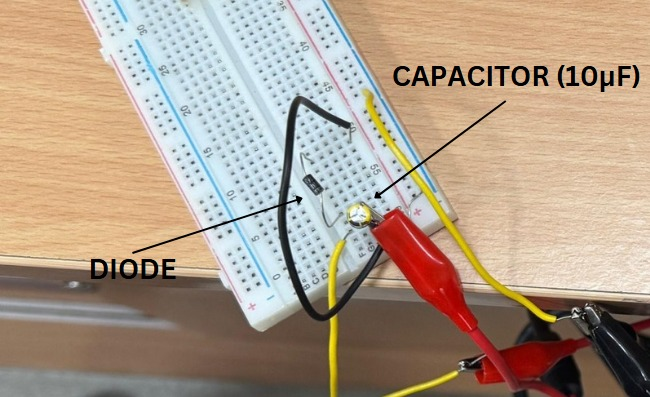
\includegraphics[width=0.7\columnwidth]{Positive_clamper.jpg}
    \caption{Positive Clamper Circuit}
    \label{fig:clamper_circuit}
\end{figure}


\begin{figure}[H]
    \centering
    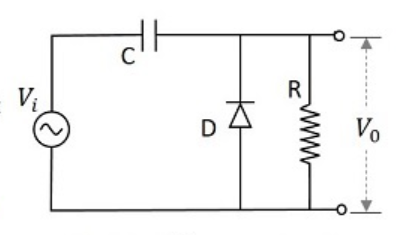
\includegraphics[width=0.7\columnwidth]{1.png}
    \caption{Positive Clamper Circuit Diagram}
    \label{fig:positive_clamper}
\end{figure}
\begin{itemize}
    \item During the \textbf{positive half cycle} of the AC input, the diode becomes \textbf{reverse-biased} because the n-side is connected to the more positive side, and the p-side is connected to the negative side/ground , As you can see in the circuit diagram.
    \item As a result, the diode does not conduct, and the capacitor charges through the input voltage to the peak value of the input.
    \item Since the diode blocks the current, the output voltage \( V_{\text{OUT}} \) is equal to the input voltage during this half-cycle
    \item During the \textbf{negative half cycle}, the diode becomes \textbf{forward-biased}, allowing current to flow through it.
    \item The capacitor, which was charged during the positive half cycle, now acts as a voltage source and shifts the input waveform upwards.
    \item This results in the entire waveform being \textbf{clamped} to a positive voltage level, effectively raising the baseline of the AC signal, As you can see in the graph below the baseline is changed from 0 to 2(because capacitor was charged upto peak voltage).
\end{itemize}
\begin{figure}[H]
    \centering
    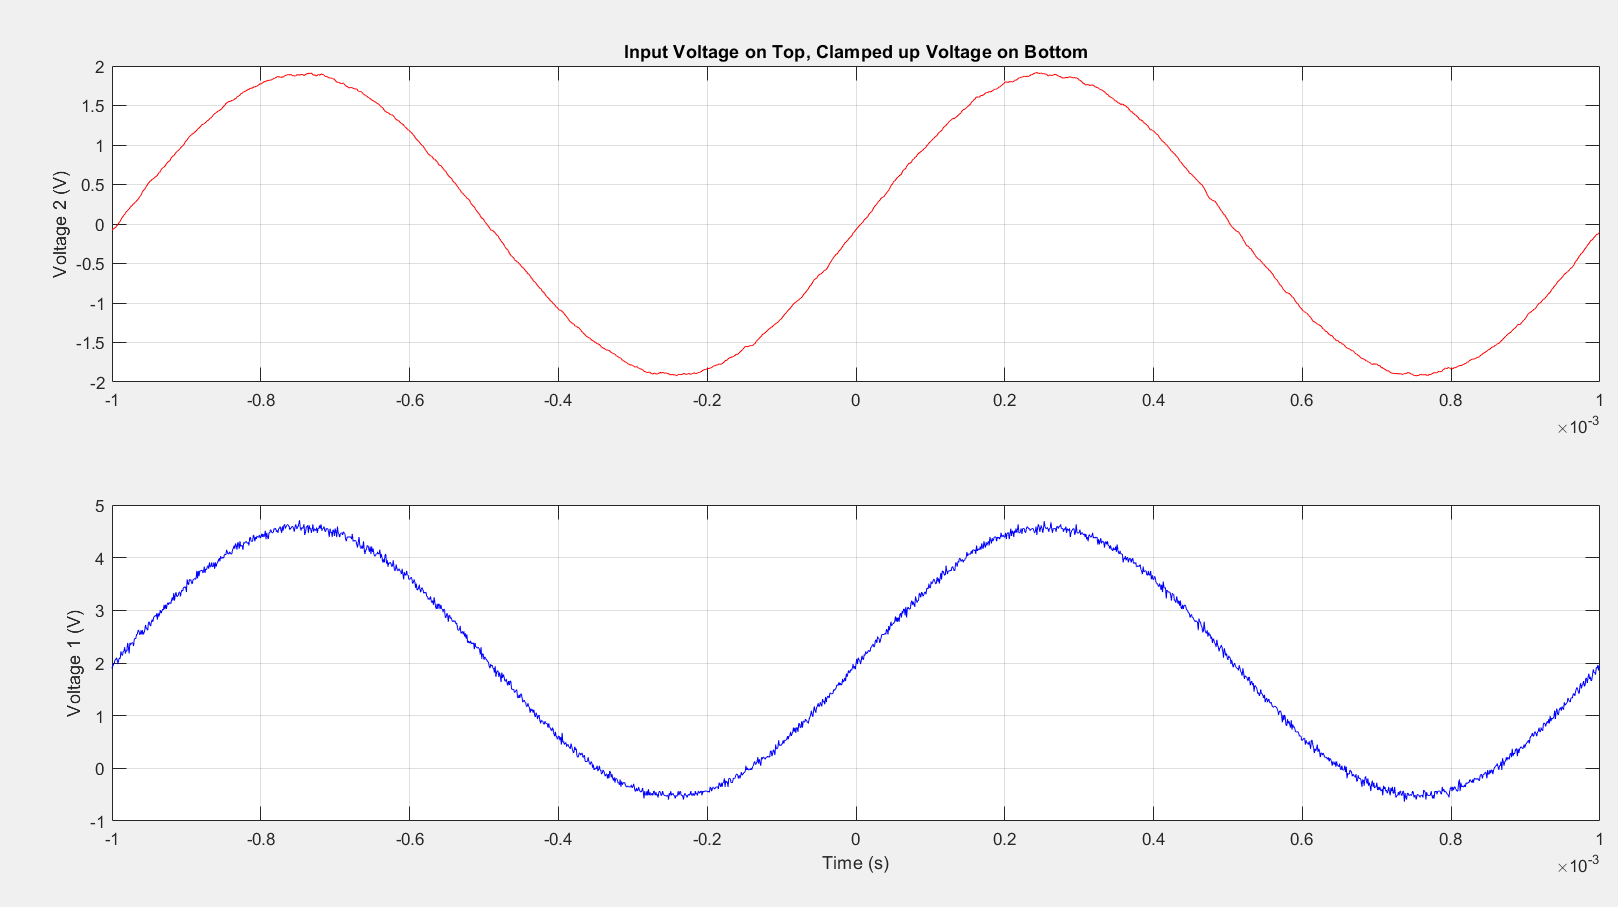
\includegraphics[width=0.7\columnwidth]{positive clamper.png}
    \caption{Positive Clamper Circuit Graph}
    \label{fig:positive_clamper}
\end{figure}

\begin{itemize}
    \item Negative clamper circuit:
\end{itemize}
\begin{figure}[H]
    \centering
    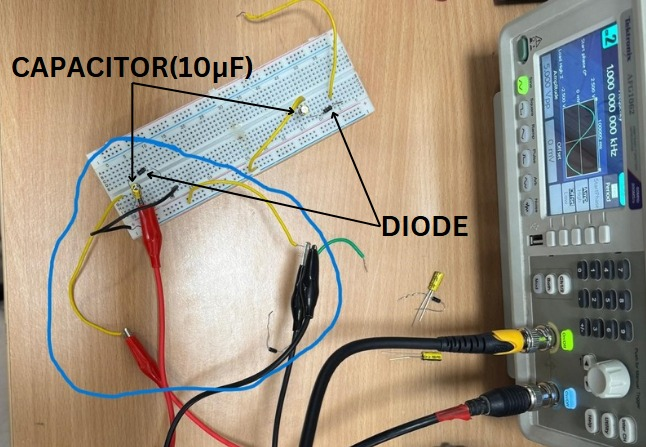
\includegraphics[width=0.7\columnwidth]{Negative_clamper.jpg}
    \caption{Negative Clamper Circuit}
    \label{fig:negative_clamper}
\end{figure}

\begin{figure}[H]
    \centering
    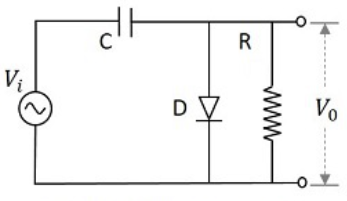
\includegraphics[width=0.7\columnwidth]{2.png}
    \caption{Negative Clamper Circuit Diagram}
    \label{fig:negative_clamper}
\end{figure}
\begin{itemize}
    \item During the \textbf{positive half cycle}, the diode is \textbf{forward-biased} because the p-side is at more positive voltage, while the n-side is connected to negative side/ground.
    \item The diode conducts, allowing the capacitor to charge to the peak input voltage but with reversed polarity compared to the positive clamper.
    \item The output voltage during this cycle is clamped near zero since the diode bypasses the input to ground.
    \item During the \textbf{negative half cycle}, the diode becomes \textbf{reverse-biased} and stops conducting.
    \item The charged capacitor now adds its voltage to the input signal, effectively shifting the entire waveform downward.
    \item This results in the waveform being \textbf{clamped} to a negative voltage level, lowering the baseline of the AC signal,As you can see in the graph below the baseline is changed from 0 to -2(because capacitor was charged upto peak voltage) .
\end{itemize}

\begin{figure}[H]
    \centering
    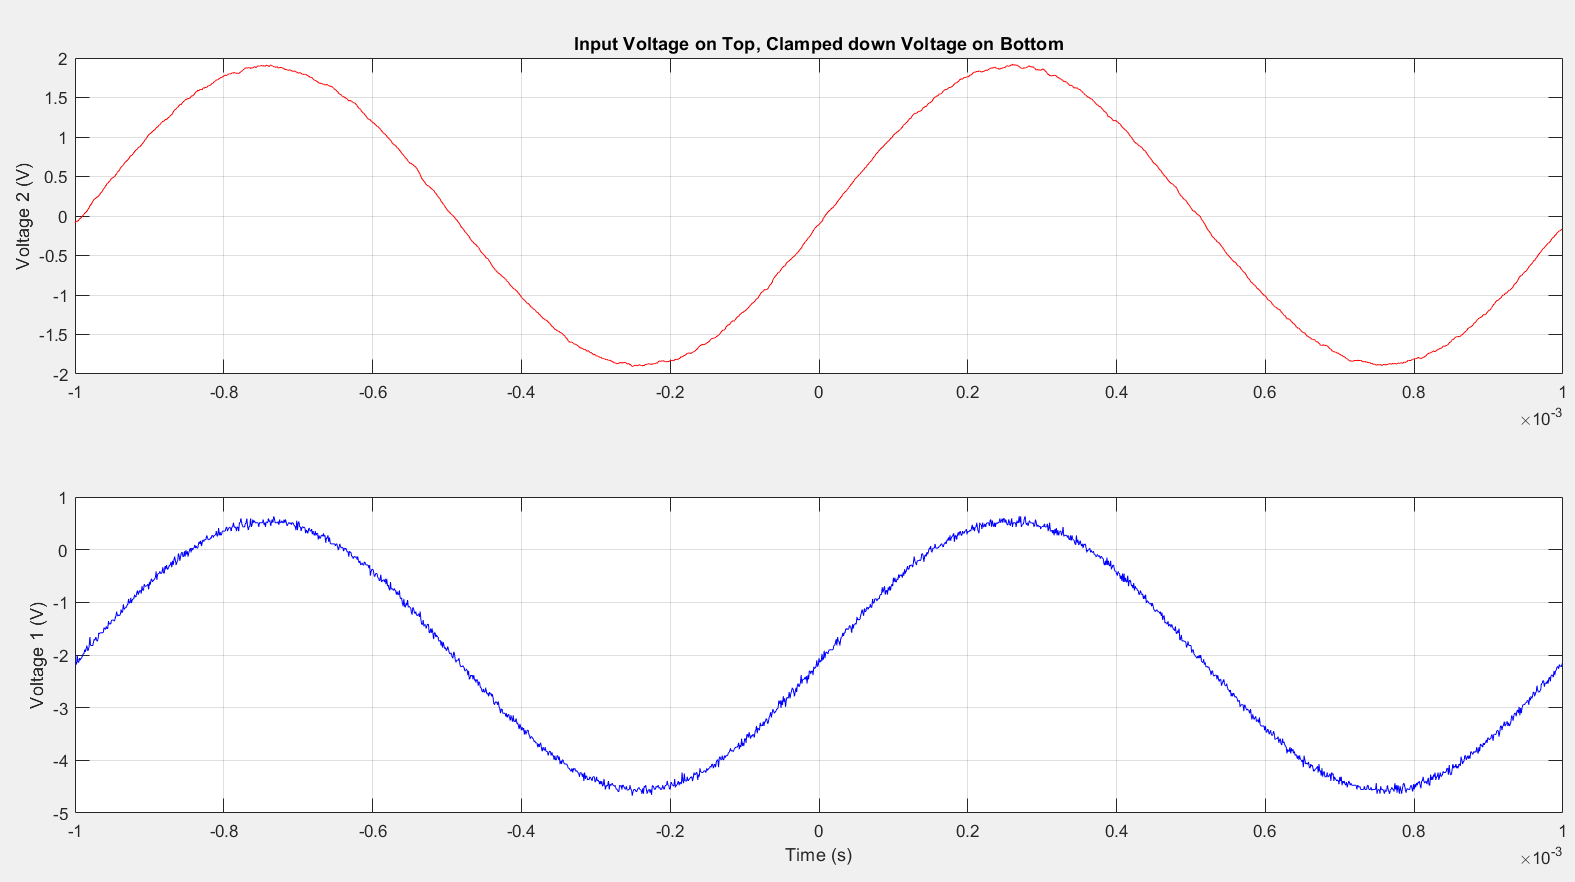
\includegraphics[width=0.7\columnwidth]{negative clamper.png}
    \caption{Negative Clamper Circuit Graph}
    \label{fig:negative_clamper}
\end{figure}



\subsection{Peak Detector Circuit}
\begin{itemize}
    \item Implemented a Peak Detector Circuit for an input voltage of 5Vpp.
    \item Positive Peak Detector Circuit:
\end{itemize}
\begin{figure}[H]
    \centering
    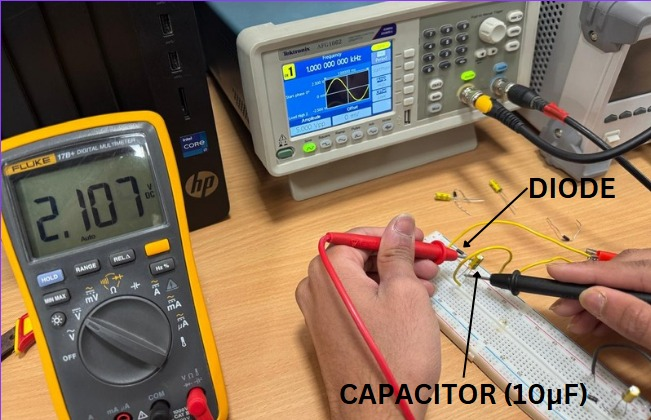
\includegraphics[width=0.7\columnwidth]{positive_peak_detector.jpg}
    \caption{Positive Peak Detector Circuit}
    \label{fig:clamper_circuit}
\end{figure}

\begin{figure}[H]
    \centering
    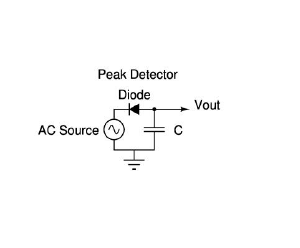
\includegraphics[width=0.7\columnwidth]{3.png}
    \caption{Positive Peak Detector circuit diagram}
    \label{fig:positive_clamper}
\end{figure}

\begin{itemize}
    \item During the \textbf{positive half cycle} of the AC input, the diode becomes \textbf{forward-biased} as the p-side is at a higher potential than the n-side.
    \item The diode conducts, allowing the capacitor \( C \) to charge up to the peak value of the input voltage minus the diode's forward voltage drop (\( V_{\text{peak}} - V_D \)).
    \item Once the capacitor is charged to the peak value, the diode becomes \textbf{reverse-biased} as the input voltage starts to decrease below the capacitor's voltage.
    \item The capacitor holds the peak voltage, and the output voltage \( V_{\text{OUT}} \) remains at the peak value since the diode prevents the capacitor from discharging back into the source.
    \item Key Point:
    \item \( V_{\text{OUT}} \approx V_{\text{peak}} - V_D \), where \( V_D \) is the forward voltage drop of the diode.
    \item Assuming an ideal diode, \( V_D = 0 \), so \( V_{\text{OUT}} = V_{\text{peak}} \).
\end{itemize}

\begin{figure}[H]
    \centering
    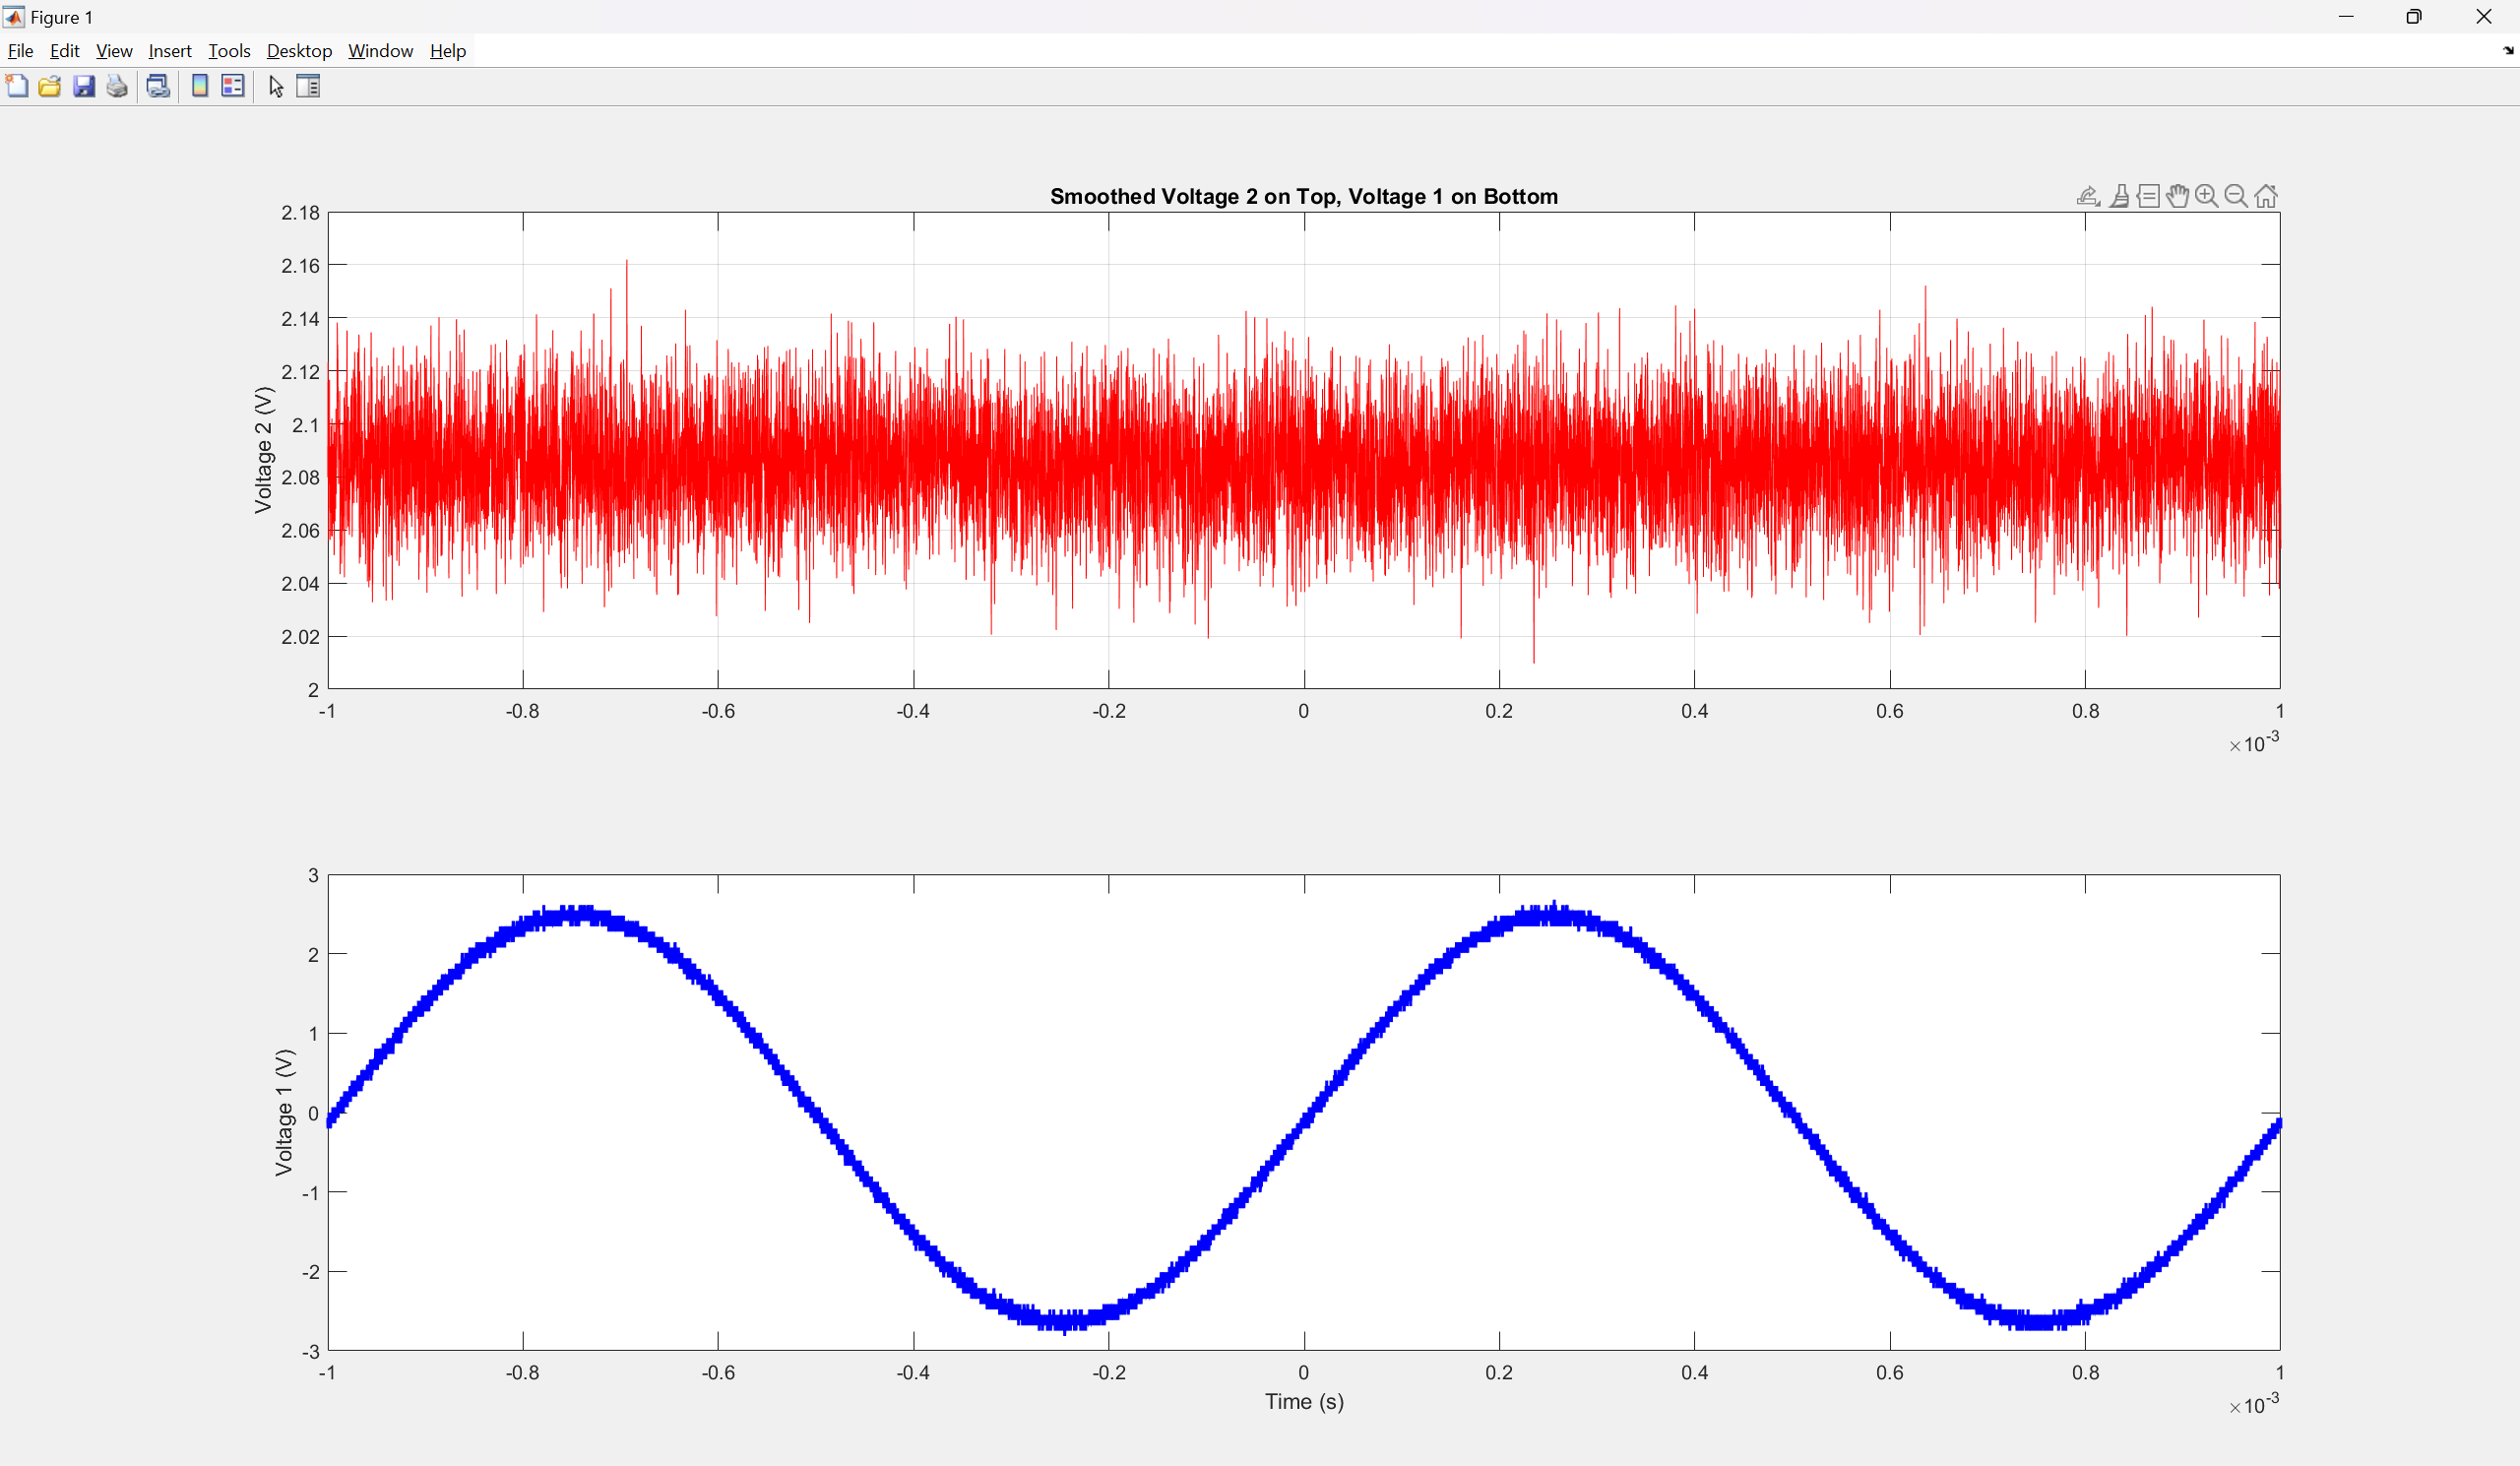
\includegraphics[width=0.7\columnwidth]{Positive_Peak_Detector.png}
    \caption{Positive Peak Detector Graph}
    \label{fig:positive_clamper}
\end{figure}


\begin{itemize}
    \item Negative Peak Detector Circuit:
\end{itemize}
\begin{figure}[H]
    \centering
    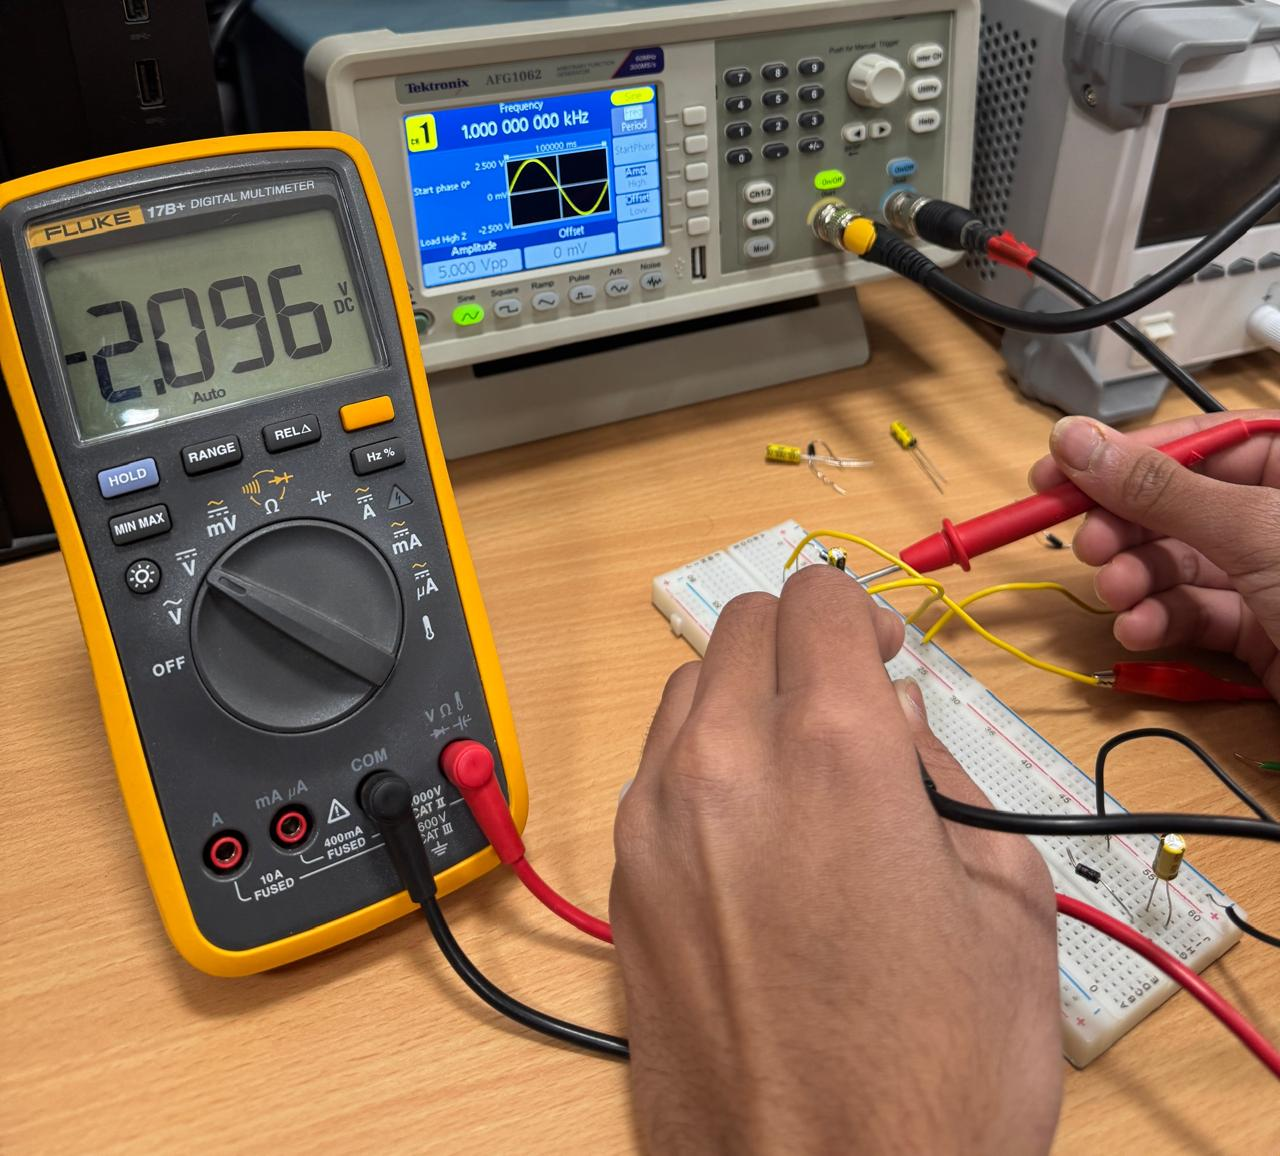
\includegraphics[width=0.7\columnwidth]{negative_peak_detector_circuit.jpg}
    \caption{Negative Peak Detector Circuit}
    \label{fig:negative_clamper}
\end{figure}
\begin{figure}[H]
    \centering
    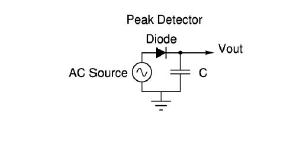
\includegraphics[width=0.7\columnwidth]{4.png}
    \caption{Negative Peak Detector Circuit Diagram}
    \label{fig:positive_clamper}
\end{figure}

\begin{itemize}
    \item During the \textbf{negative half cycle} of the AC input, the diode becomes \textbf{forward-biased} as the cathode is at a lower potential than the anode.
    \item The diode conducts, and the capacitor \( C \) charges to the negative peak value of the input voltage (\( V_{\text{peak}}^{-} + V_D \)).
    \item As the input voltage starts rising back toward zero, the diode becomes \textbf{reverse-biased}, preventing the capacitor from discharging.
    \item The capacitor holds the most negative peak, and the output voltage \( V_{\text{OUT}} \) stays at that value.
    \item Key Point:
    \item \( V_{\text{OUT}} \approx V_{\text{peak}}^{-} + V_D \), where \( V_D \) is the diode's forward voltage drop.
    \item For an ideal diode, \( V_D = 0 \), resulting in \( V_{\text{OUT}} = V_{\text{peak}}^{-} \).
\end{itemize}

\begin{figure}[H]
    \centering
    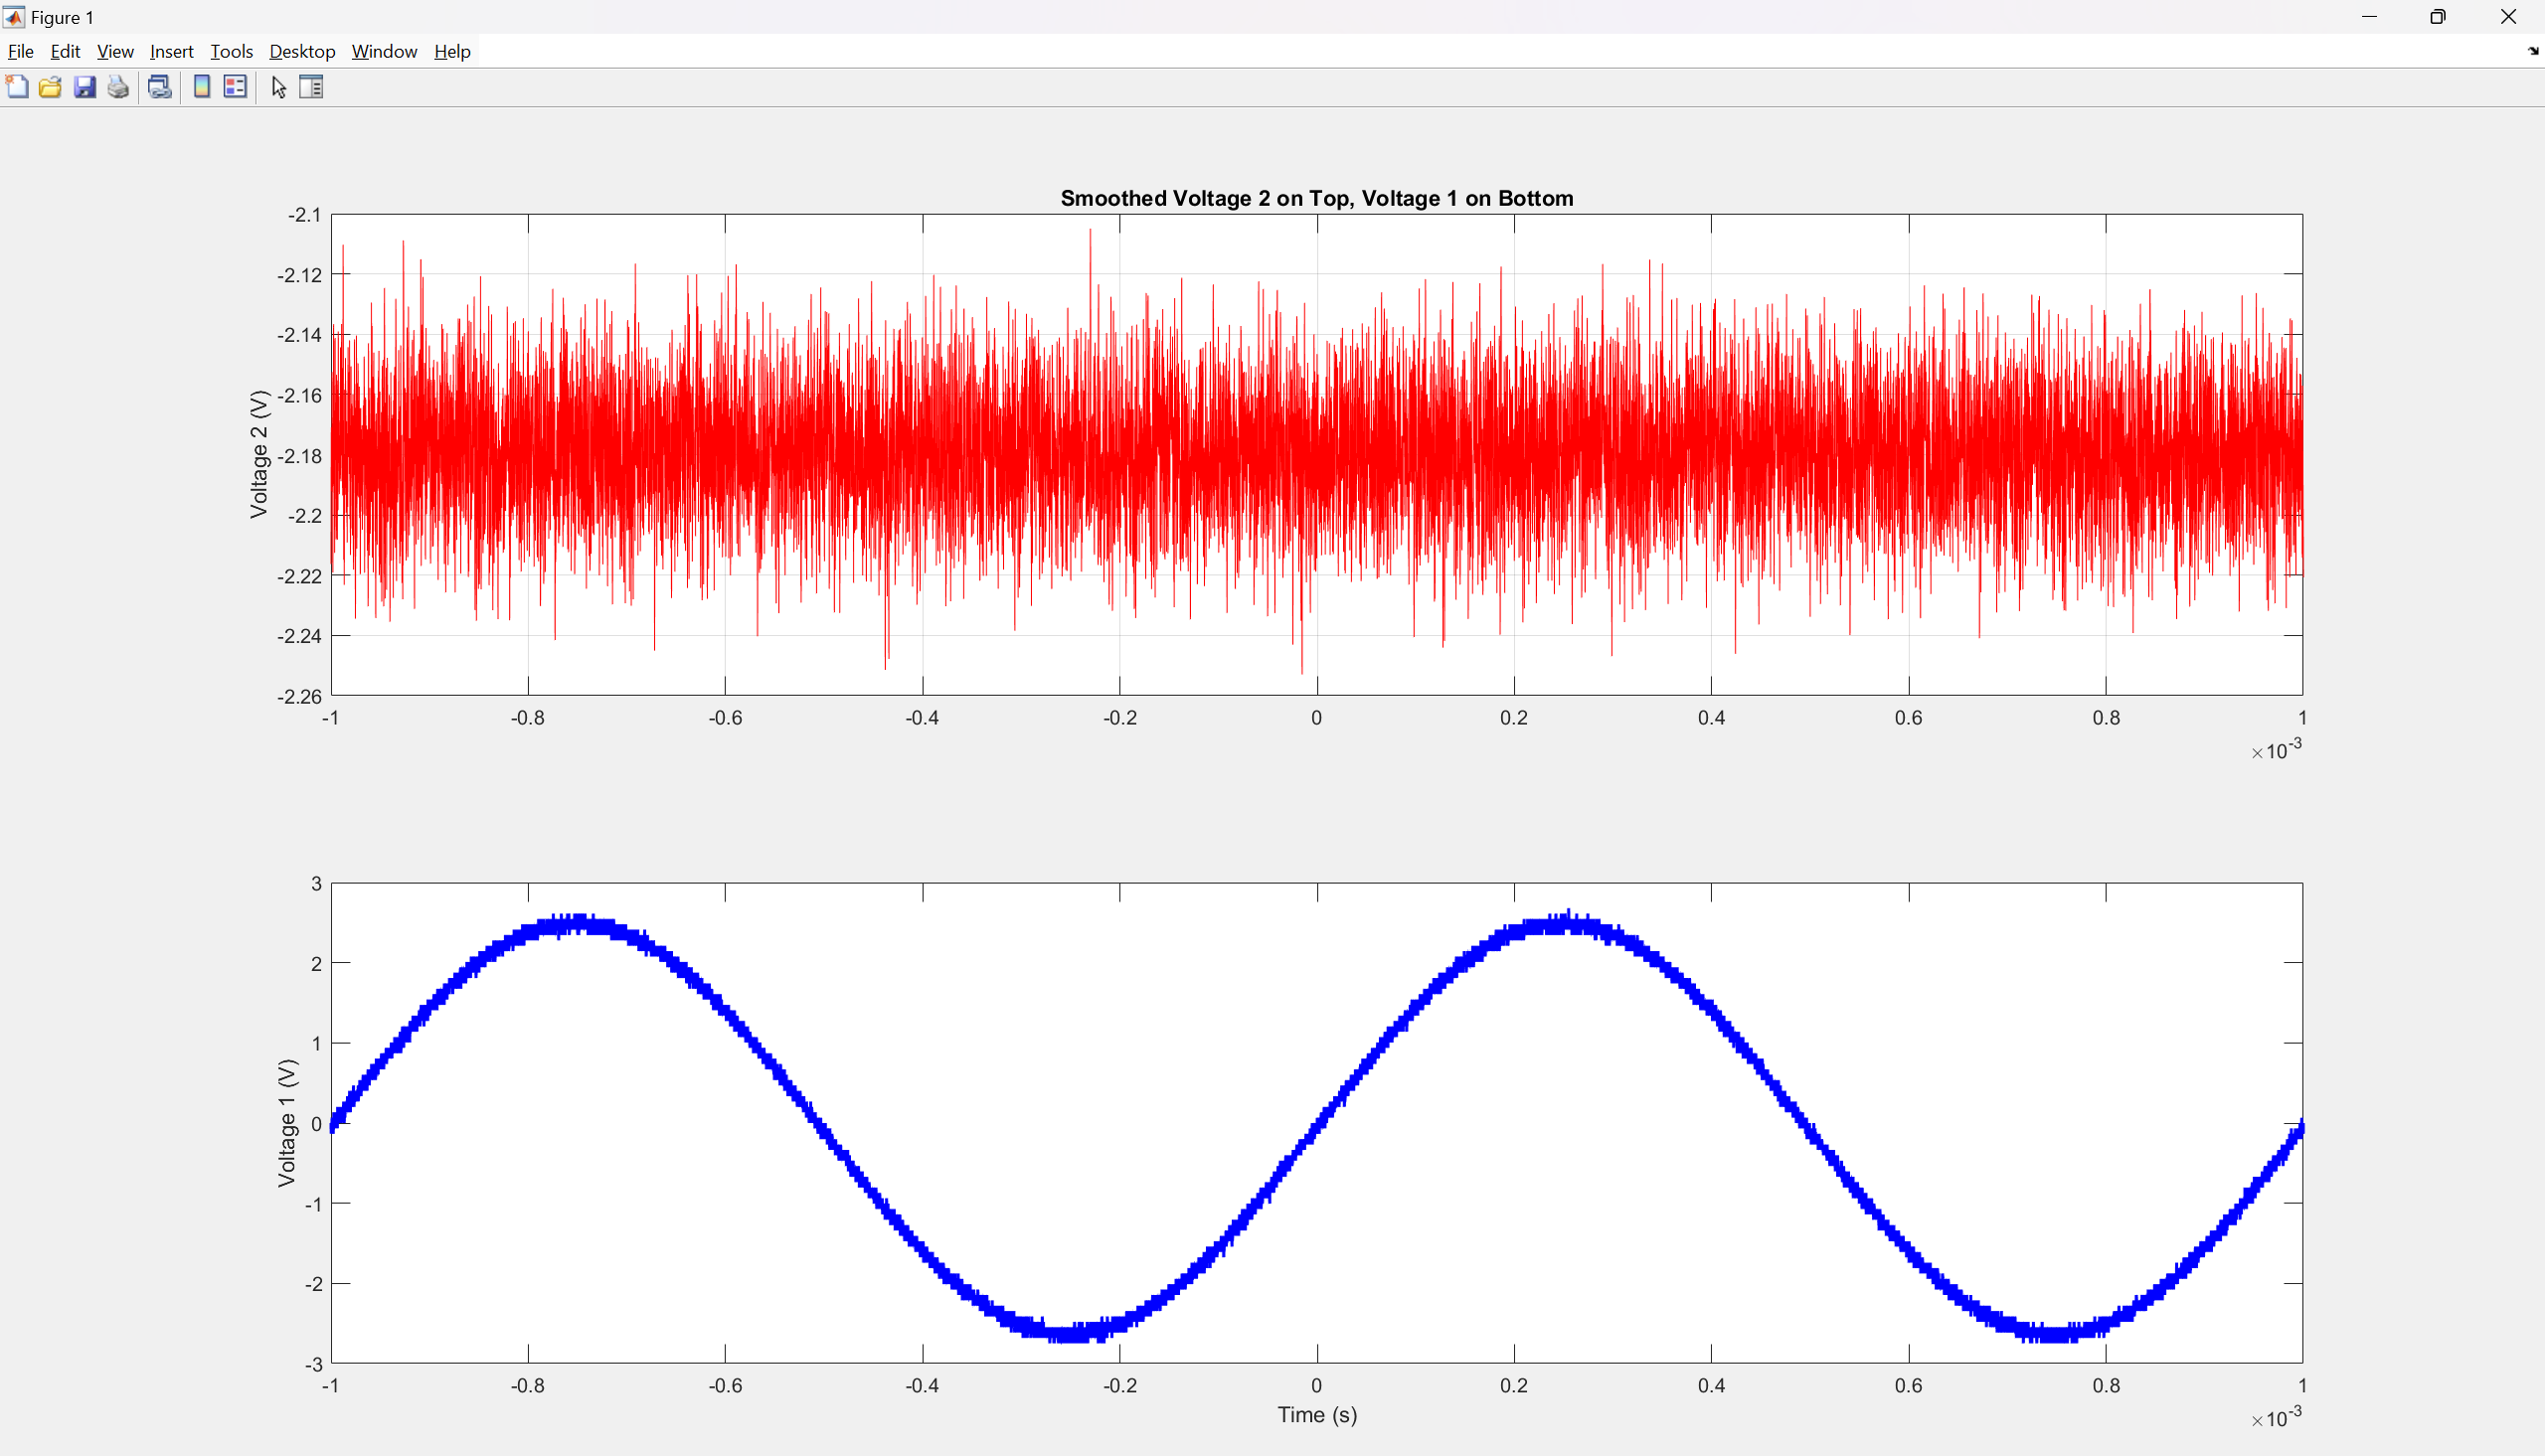
\includegraphics[width=0.7\columnwidth]{Negative_peak_detector.png}
    \caption{Negative Peak Detector Graph}
    \label{fig:positive_clamper}
\end{figure}


\subsection{Voltage Doubler Circuit}
\begin{itemize}
    \item Implemented a voltage Doubler Circuit for an input voltage of 4Vpp.
\end{itemize}
\begin{figure}[H]
    \centering
    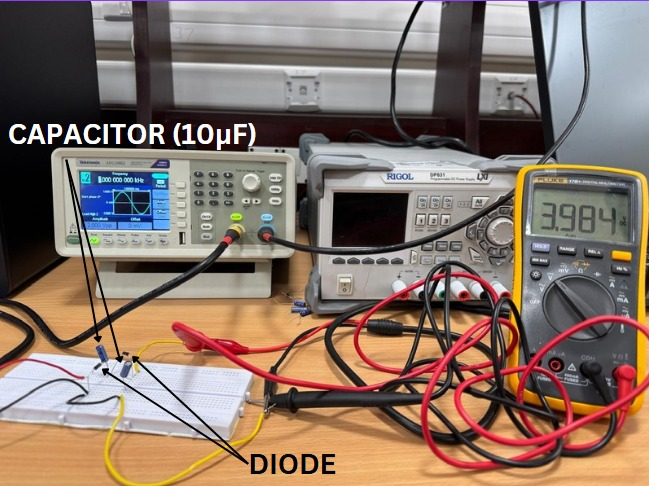
\includegraphics[width=0.7\columnwidth]{Voltage_Doubler.jpg}
    \caption{Voltage Doubler Circuit}
    \label{fig:negative_clamper}
\end{figure}
\begin{itemize}
    \item As you can see we gave 4Vpp(peak is 2V) so by implementing the voltage doubler circuit we got output voltage double to the input voltage i.e 4V(approx)
\end{itemize}
\begin{figure}[H]
    \centering
    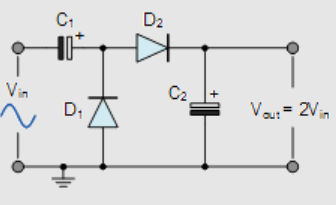
\includegraphics[width=0.7\columnwidth]{5.png}
    \caption{Voltage Doubler Circuit Diagram}
    \label{fig:positive_clamper}
\end{figure}
\begin{itemize}
    \item The voltage doubler circuit uses two diodes and two capacitors to double the peak voltage of the AC input.
    \item During the \textbf{negative half cycle} of the AC input:
    \begin{itemize}
        \item The first diode becomes \textbf{forward-biased}, charging the first capacitor \( C_1 \) to the peak input voltage \( V_{\text{peak}} \).
    \end{itemize}
    \item During the \textbf{positive half cycle}:
    \begin{itemize}
        \item The second diode becomes \textbf{forward-biased}, and the second capacitor \( C_2 \) charges using the voltage from the AC source and \( C_1 \), effectively doubling the voltage.
    \end{itemize}
    \item The output voltage \( V_{\text{OUT}} \) across \( C_2 \) becomes approximately \( 2V_{\text{peak}} \) (neglecting diode drops), As you can see in the graph below we get a straight line at 4V(approximately, since diode is not ideal).
    \item Key Point:
    \begin{itemize}
        \item \( V_{\text{OUT}} \approx 2V_{\text{peak}} \) in an ideal case.
        \item The circuit is commonly used in applications requiring higher DC voltages from lower AC sources. 
    \end{itemize}
\end{itemize}
\begin{figure}[H]
    \centering
    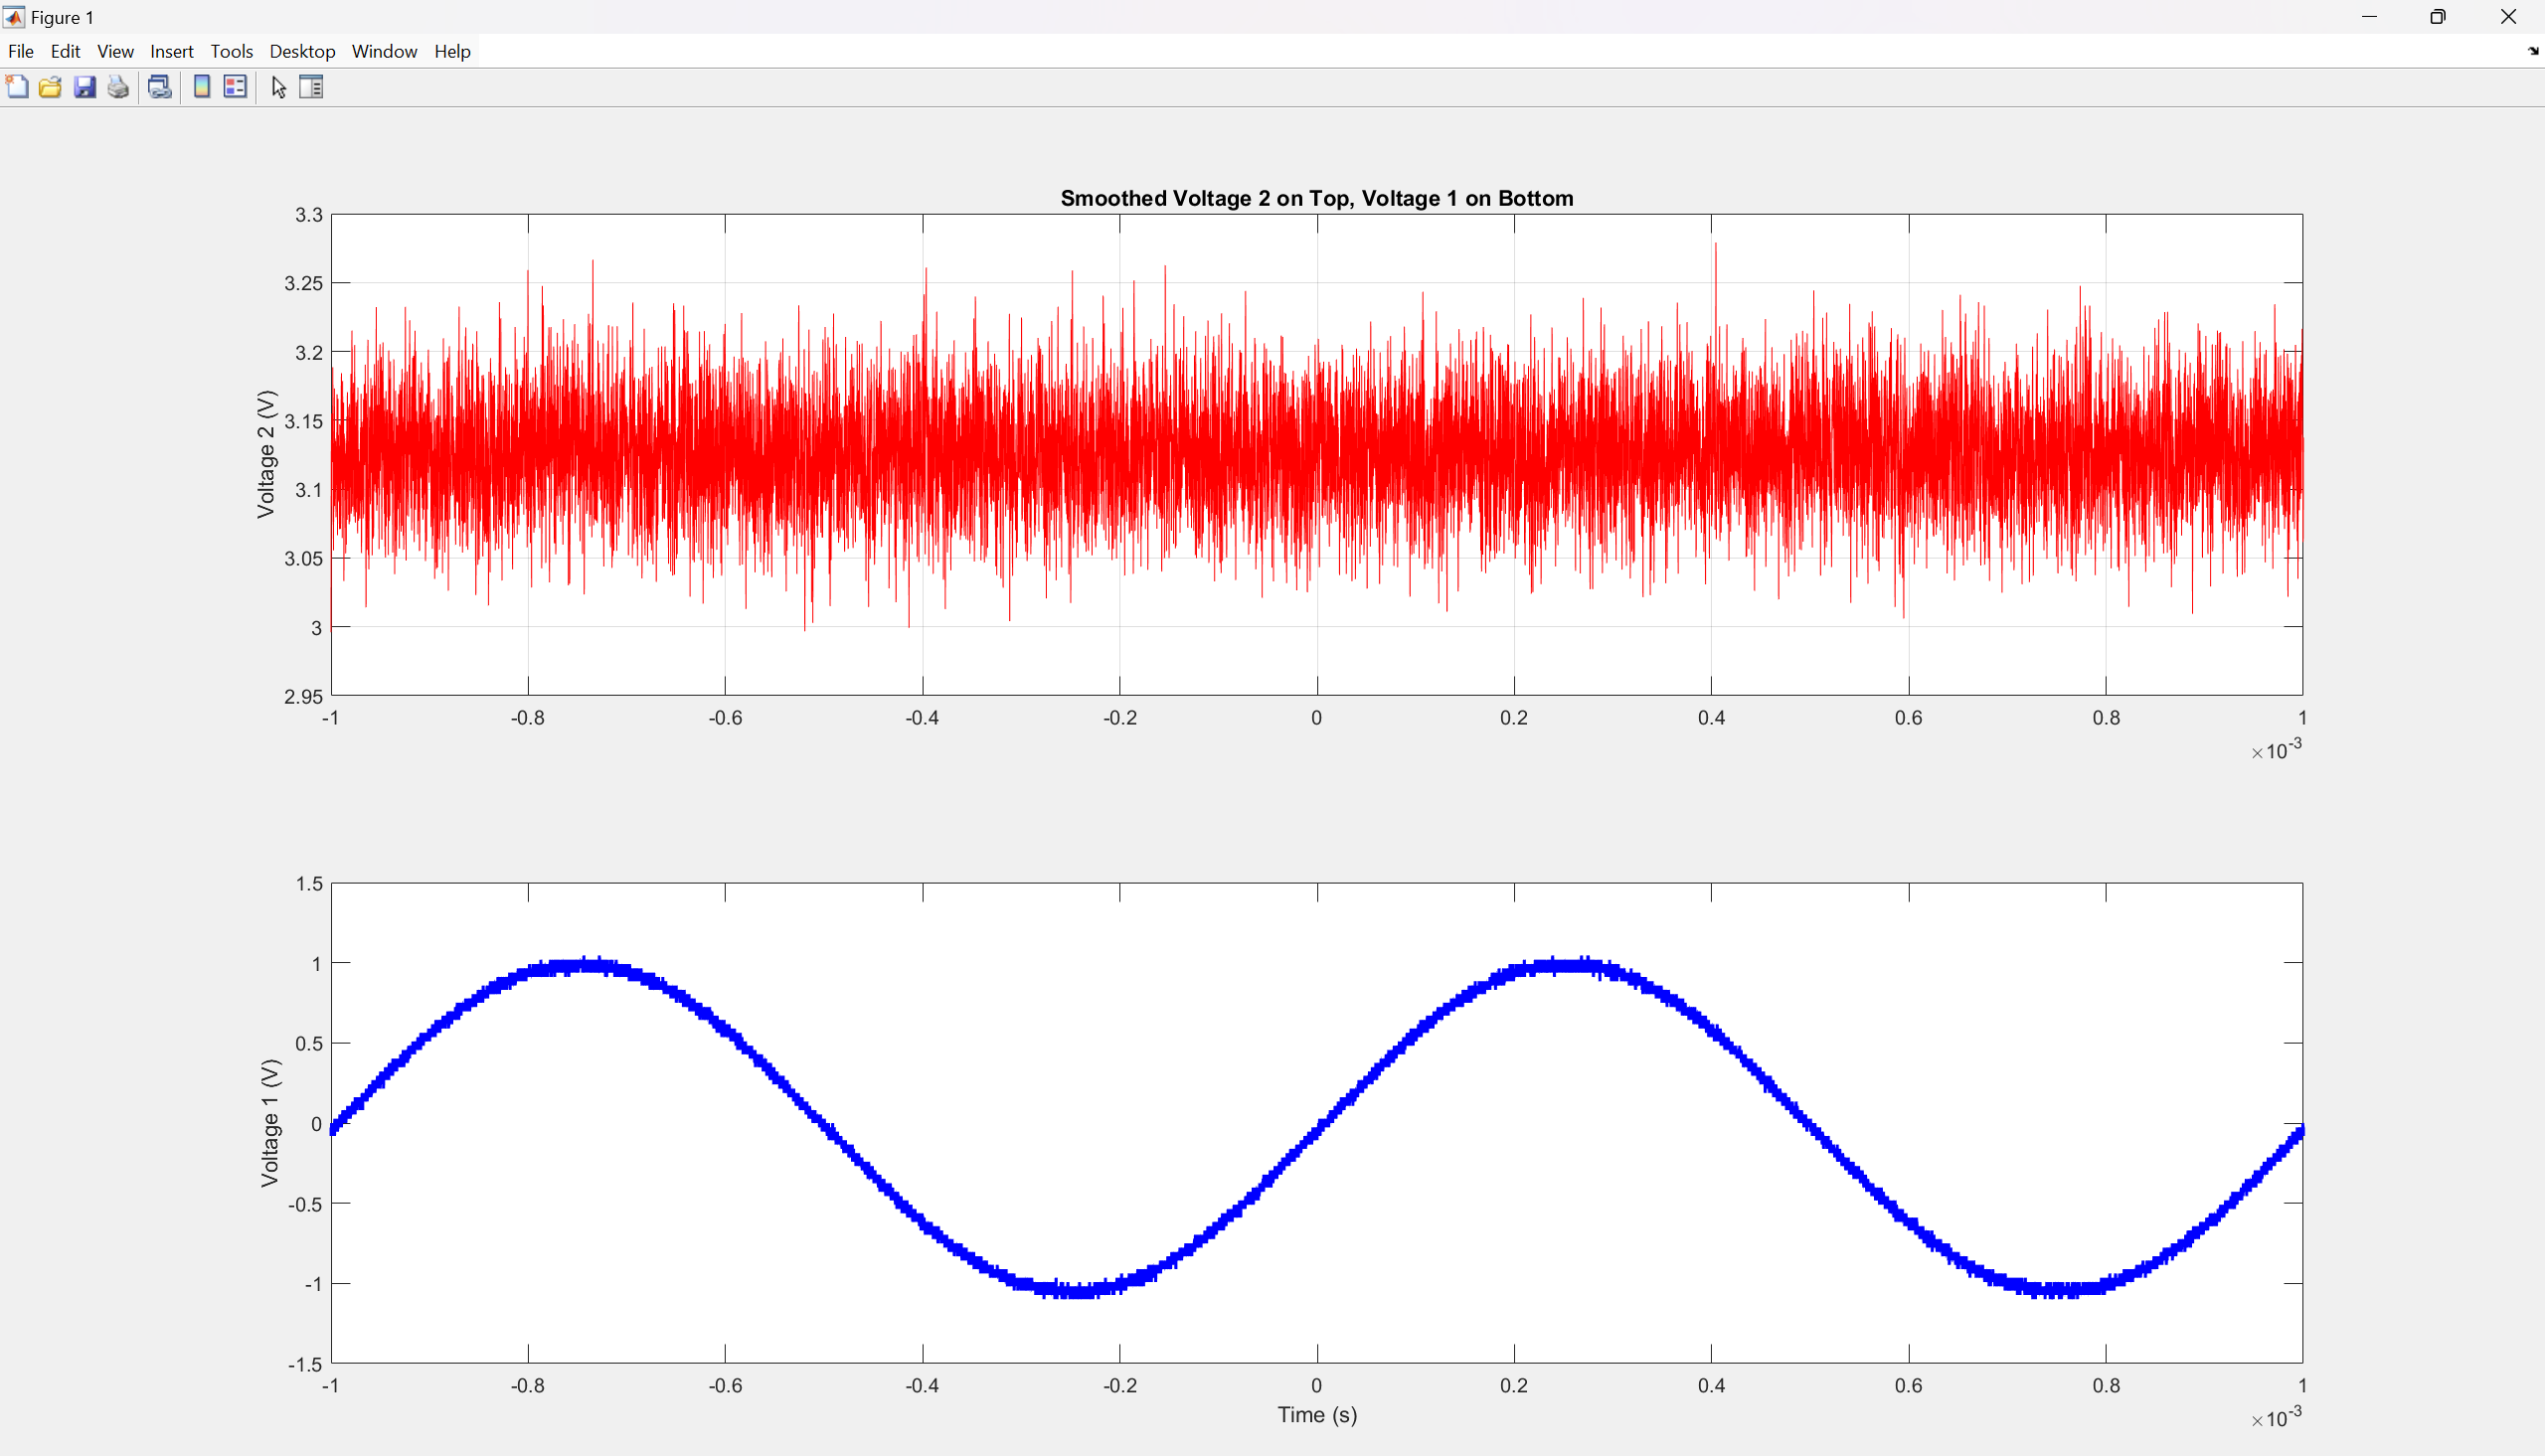
\includegraphics[width=0.7\columnwidth]{Doubler.png}
    \caption{Voltage Doubler Graph}
    \label{fig:positive_clamper}
\end{figure}


\subsection{Voltage Quadruple}
\begin{itemize}
    \item Implemented a voltage Quadruple Circuit for an input voltage of 5Vpp.
\end{itemize}
\begin{figure}[H]
    \centering
    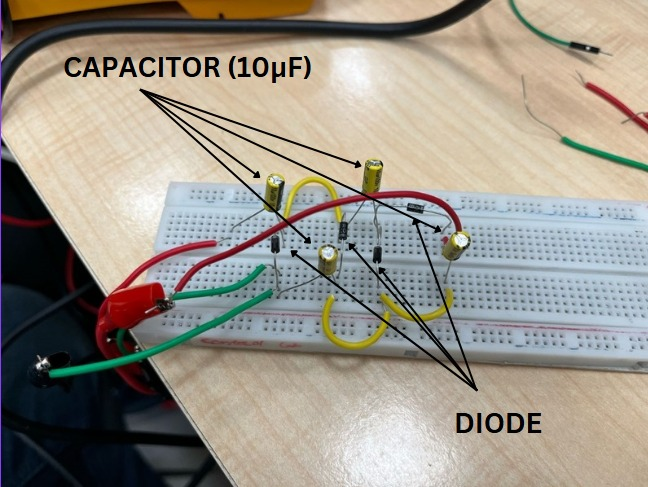
\includegraphics[width=0.7\columnwidth]{Voltage_quadruple.jpg}
    \caption{Voltage Quadruple Circuit}
    \label{fig:negative_clamper}
\end{figure}

\begin{itemize}
    \item As you can see we gave 5Vpp(peak is 2.5V) so by implementing the voltage quadruple circuit we got output voltage four times to the input voltage i.e 10V(approx)
\end{itemize}
\begin{figure}[H]
    \centering
    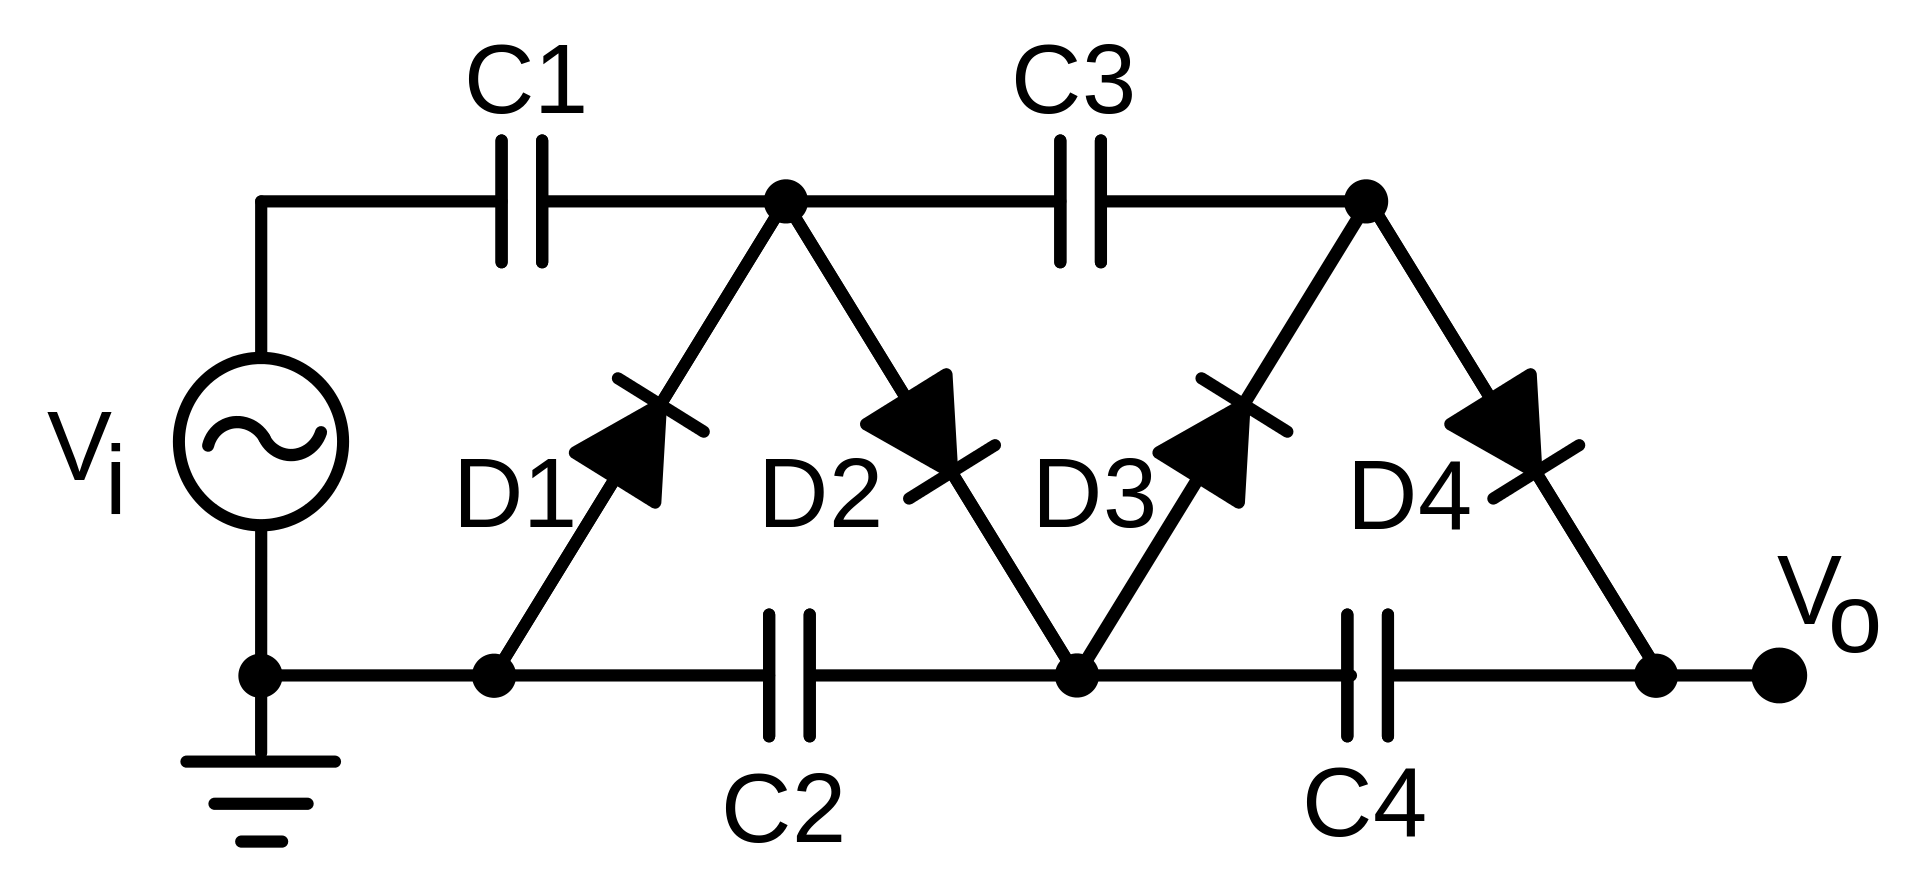
\includegraphics[width=0.7\columnwidth]{6.png}
    \caption{Voltage Quadruple Circuit Diagram}
    \label{fig:positive_clamper}
\end{figure}

\begin{itemize}
    \item The voltage quadrupler extends the voltage doubler principle by using four diodes and four capacitors.
    \item During alternate half cycles:
    \begin{itemize}
        \item Capacitors charge sequentially, each adding \( V_{\text{peak}} \) to the total output.
        \item The diodes direct the current in such a way that each capacitor adds its voltage to the next stage.
    \end{itemize}
    \item The final output voltage \( V_{\text{OUT}} \) across the last capacitor is approximately \( 4V_{\text{peak}} \), As you can see in the graph below we get a straight line at 10V(approximately, since diode is not ideal).
    \item Key Point:
    \begin{itemize}
        \item \( V_{\text{OUT}} \approx 4V_{\text{peak}} \) in an ideal case.
        \item Voltage quadruplers are used in applications that require high DC voltages without using a transformer.
    \end{itemize}
\end{itemize}
\begin{figure}[H]
    \centering
    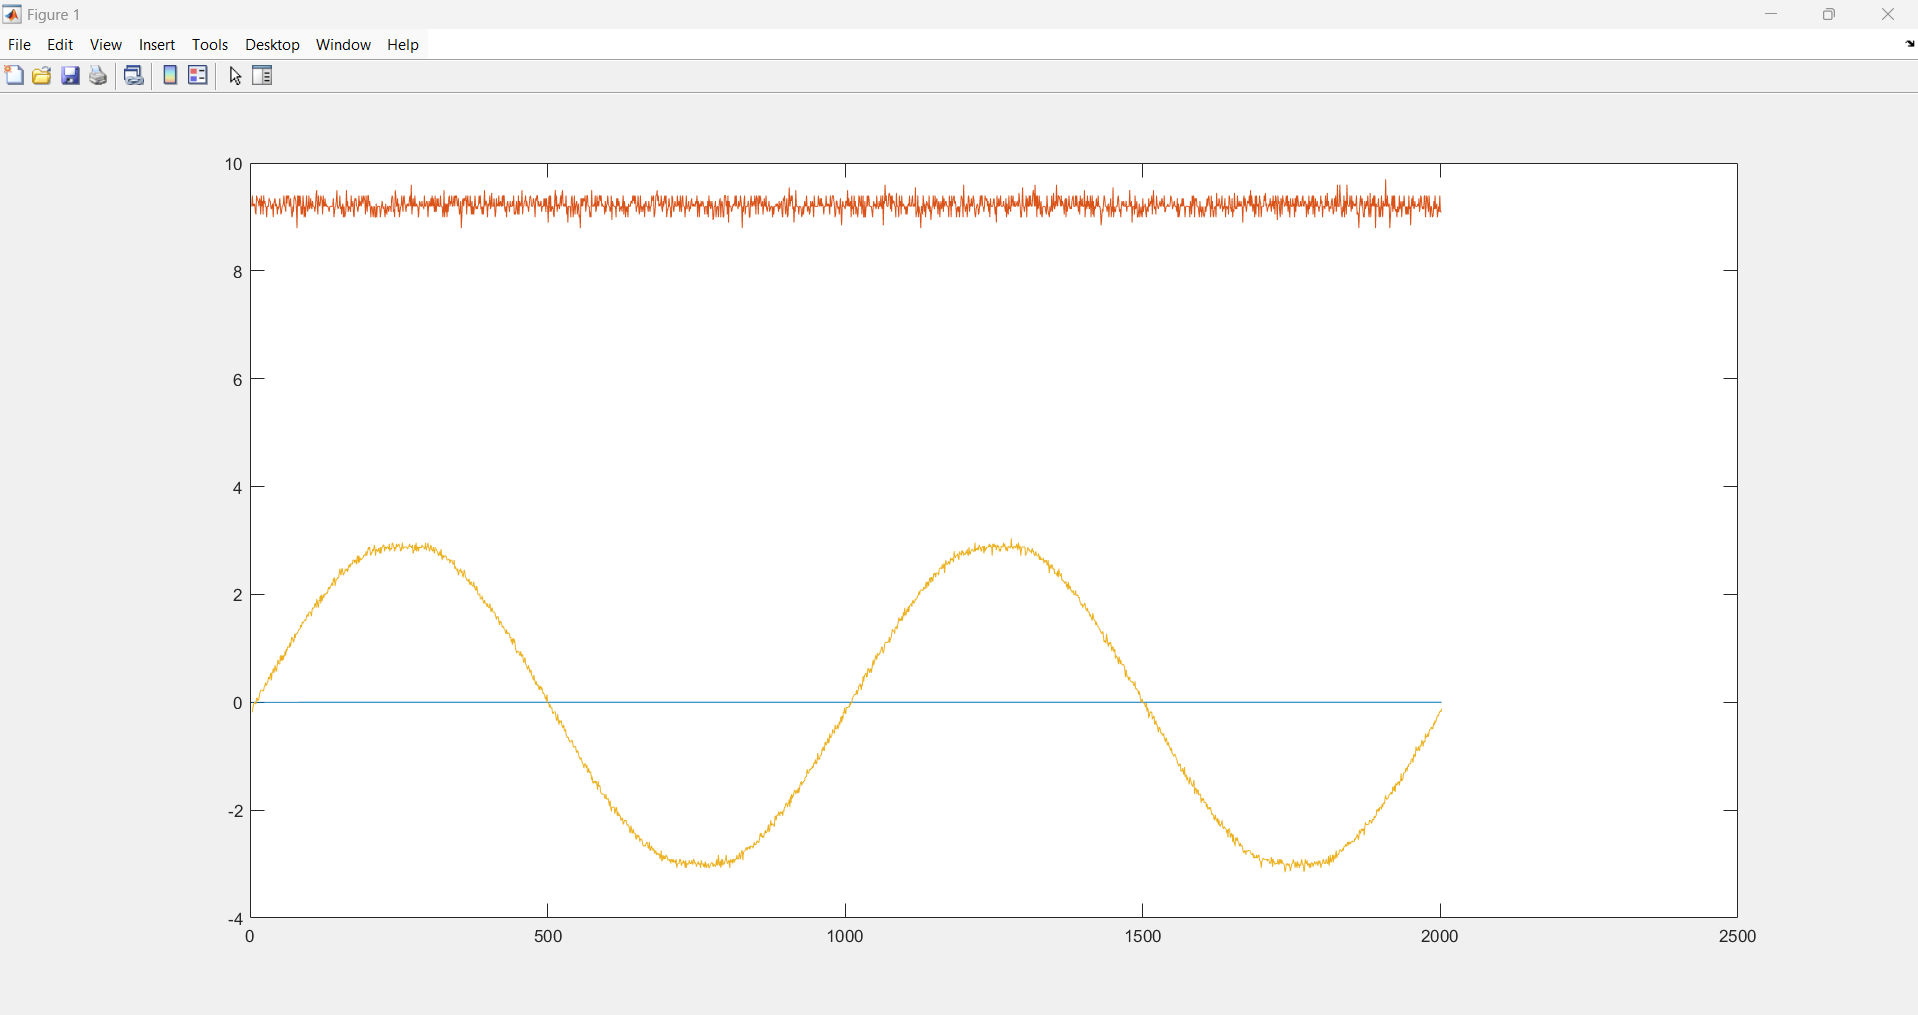
\includegraphics[width=0.7\columnwidth]{quadrupler.png}
    \caption{Voltage Quadruple Graph}
    \label{fig:positive_clamper}
\end{figure}



\section{Discussion}
\begin{itemize}
    \item A voltage drop is observed in the peak detector and voltage multiplier circuits, which deviates from theoretical expectations.
    \item The key reasons for this voltage drop include:
    \begin{itemize}
        \item \textbf{Diode Forward Voltage Drop}: The silicon diodes used (such as 1N4007) have a forward voltage drop (~0.7V), which accumulates over multiple stages.
        \item \textbf{Capacitor Leakage and ESR}: Non-ideal capacitors exhibit leakage current and Equivalent Series Resistance (ESR), leading to charge loss and reduced voltage storage.
        \item \textbf{Load Resistance Effects}: The presence of the multimeter or other connected loads can drain charge from the circuit, resulting in a lower measured voltage.
        \item \textbf{Frequency Dependence}: At improper input signal frequencies, capacitors may not fully charge or discharge, reducing peak output voltage.
        \item \textbf{Parasitic Effects}: Wire resistance, PCB trace inductance, and stray capacitance contribute to energy loss in the circuit.
        \item \textbf{Temperature Variation}: The forward voltage drop of diodes decreases with temperature (~2mV/°C), causing slight variations in output voltage.
        \item \textbf{Measurement Errors}: Multimeter impedance and oscilloscope probe characteristics can introduce minor inaccuracies in the observed voltage values.
    \end{itemize}
\end{itemize}


\section{Conclusion}
\noindent{The implementation of voltage multipliers using clamper and peak detector circuits was successfully carried out, and the results were observed to be in agreement with theoretical expectations, with some minor deviations due to practical circuit limitations.}\\

\section{References}
\begin{enumerate}
    \item Fundamentals of Microelectronics by Behzad Razavi
    \item Microelectronic circuits by Adel Sedra and Kenneth Smith
\end{enumerate}

\end{document}
